\documentclass[12pt]{article}
\usepackage{amsmath, amssymb}
\usepackage{geometry}
\usepackage{fancyhdr}
\usepackage{pgfplots}
\pgfplotsset{compat=1.18}
\usepackage{multicol}

\geometry{margin=1in}
\pagestyle{fancy}
\fancyhf{}
\rhead{Name: \underline{\hspace{2in}}}
\lhead{Piecewise Functions - Guided Notes}
\cfoot{\thepage}

\usepackage{tgadventor}
\renewcommand*\familydefault{\sfdefault} %% Only if the base font of the document is to be sans serif
\usepackage[T1]{fontenc}

\title{Introduction to Piecewise Functions}
\date{}

\begin{document}

%\maketitle

\subsection*{What is a Piecewise Function?}

A \textbf{piecewise function} is a function that is defined by \textbf{different expressions} that depend on the value of the input ($x$).

\vspace{0.5cm}

\noindent
\textbf{Example:}
\[
f(x) = 
\begin{cases}
x + 2 & \text{if } x < 0 \\
x^2 & \text{if } x \geq 0
\end{cases}
\]

\textbf{This means:}
\begin{itemize}
  \item If $x$ is \underline{\hspace{2in}} 0 then use the rule $f(x) = x + 2$
  \item If $x$ is \underline{\hspace{3.5in}} 0 then use the rule $f(x) = x^2$
\end{itemize}

\vspace{0.3cm}

\noindent\textbf{Try evaluating:}

\begin{itemize}
  \item $f(-3) = $ \underline{\hspace{1in}}
  \item $f(0) = $ \underline{\hspace{1in}}
  \item $f(2) = $ \underline{\hspace{1in}}
\end{itemize}

\vspace{0.5cm}

\subsection*{Graphing a Piecewise Function}

To graph a piecewise function:

\begin{enumerate}
  \item Look at each piece separately.
  \item Graph that part only on the interval where it applies.
  \item Use open or closed circles to show whether endpoints are included.
\end{enumerate}

\vspace{0.3cm}

\noindent
\textbf{Example:}
\[
g(x) = 
\begin{cases}
2x + 1 & \text{if } x \leq 1 \\
-1 & \text{if } x > 1
\end{cases}
\]

\begin{center}
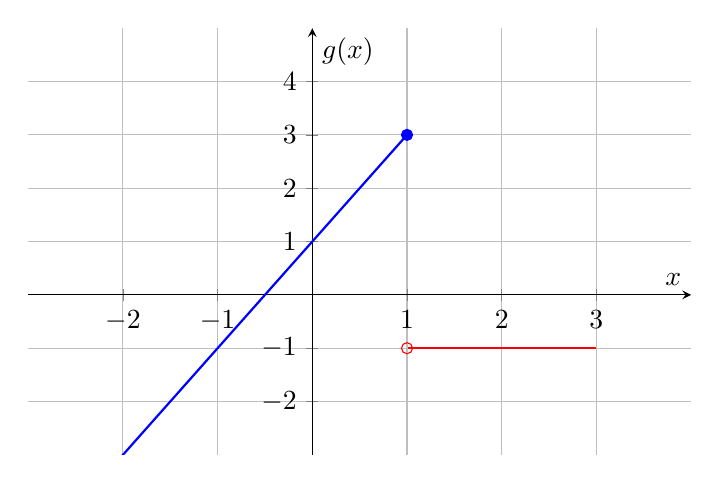
\begin{tikzpicture}
\begin{axis}[
    axis lines = center,
    xmin=-3, xmax=4,
    ymin=-3, ymax=5,
    xtick={-2,-1,0,1,2,3},
    ytick={-2,-1,0,1,2,3,4},
    width=10cm,
    height=7cm,
    samples=100,
    domain=-3:3,
    xlabel=$x$, ylabel=$g(x)$,
    grid=both
]

% Line segment for 2x + 1 where x <= 1
\addplot[
    domain=-3:1,
    blue,
    thick
]{2*x + 1};

% Constant function where x > 1
\addplot[
    domain=1.01:3,
    red,
    thick
]{-1};

% Closed dot at x=1 for 2x+1
\addplot[only marks, mark=*, blue] coordinates {(1,3)};
% Open dot at x=1 for -1
\addplot[only marks, mark=o, red] coordinates {(1,-1)};

\end{axis}
\end{tikzpicture}
\end{center}

\vspace{0.5cm}

\section*{Your Turn!}

\noindent
Here’s a piecewise function for you to evaluate and sketch:

\[
h(x) = 
\begin{cases}
2x-1 & \text{if } x < 2 \\
 1 & \text{if } x \geq 2
\end{cases}
\]

\begin{itemize}
  \item $h(1) = $ \underline{\hspace{1in}}
  \item $h(2) = $ \underline{\hspace{1in}}
  \item $h(3) = $ \underline{\hspace{1in}}
\end{itemize}

\vspace{0.3cm}

\begin{center}
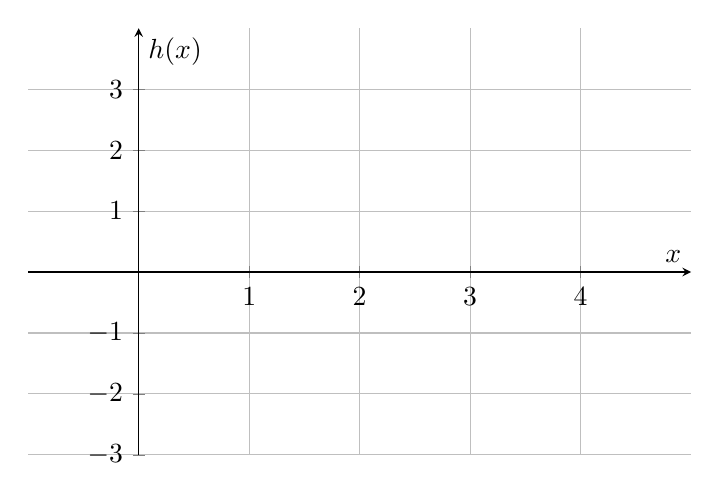
\begin{tikzpicture}
\begin{axis}[
    axis lines = center,
    xmin=-1, xmax=5,
    ymin=-3, ymax=4,
    xtick={0,1,2,3,4},
    ytick={-3,-2,-1,0,1,2,3},
    width=10cm,
    height=7cm,
    samples=100,
    domain=0:4,
    xlabel=$x$, ylabel=$h(x)$,
    grid=both
]
\end{axis}
\end{tikzpicture}
\end{center}

Here is another function 
\[
k(x) = 
\begin{cases}
  \frac{1}{2}x+1 & \text{if } x < 2 \\
  x+1 & \text{if } x \geq 2
\end{cases}
\]

\begin{itemize}
  \item $k(1) = $ \underline{\hspace{1in}}
  \item $k(2) = $ \underline{\hspace{1in}}
  \item $k(3) = $ \underline{\hspace{1in}}
\end{itemize}

\vspace{0.3cm}

\begin{center}
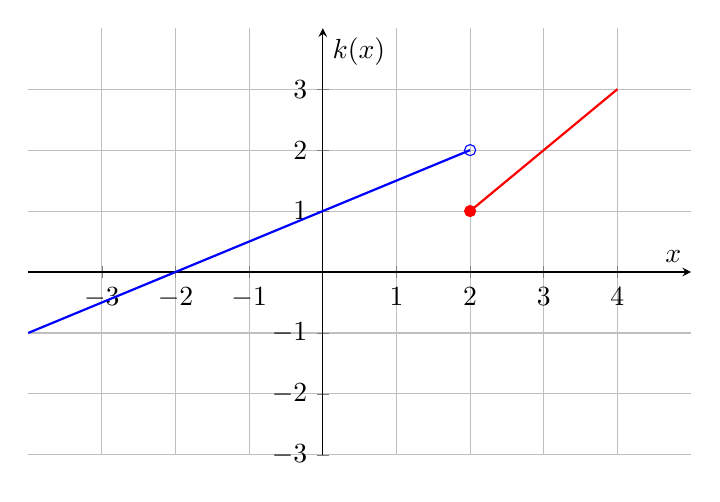
\begin{tikzpicture}
\begin{axis}[
    axis lines = center,
    xmin=-4, xmax=5,
    ymin=-3, ymax=4,
    xtick={-3,-2,-1,0,1,2,3,4},
    ytick={-3,-2,-1,0,1,2,3},
    width=10cm,
    height=7cm,
    samples=100,
    domain=0:4,
    xlabel=$x$, ylabel=$k(x)$,
    grid=both
]

% Line segment for 2x + 1 where x <= 1
\addplot[
    domain=-4:2,
    blue,
    thick
]{0.5*x + 1};

% Constant function where x > 1
\addplot[
    domain=2.01:4,
    red,
    thick
]{x-1};

% Closed dot at x=1 for 2x+1
\addplot[only marks, mark=o, blue] coordinates {(2,2)};
% Open dot at x=1 for -1
\addplot[only marks, mark=*, red] coordinates {(2,1)};

\end{axis}
\end{tikzpicture}
\end{center}

\end{document}

